\documentclass[11pt]{article}
\usepackage{hyperref}
\usepackage{hyperref}
\usepackage[backend=biber,
  natbib=true,
  style=numeric,
  sorting=nyt]{biblatex}
\addbibresource{defs.bib}
\addbibresource{arrpubs.bib}
\addbibresource{molrec.bib}
\usepackage[letterpaper,margin=1in]{geometry}
\usepackage{verbatim,moreverb}
\usepackage{graphicx}
\begin{document}
\title{An Msprime Tutorial}
\author{Alan R. Rogers}
\date{\today}
\maketitle

\section{Introduction}
\label{sec.intro}
In this project, you will use msprime \citep{Kelleher:PLO-12-1} to
check for bias in the estimates from your Legofit project. This will
involve the following steps:
\begin{enumerate}
\item Install msprime on your computer.
\item Modify the Python script described below, so that it simulates
  your own model of history.
\item Run the script to generate simulated data, and pipe the output
  into simpat, from the Legofit package, to generate site pattern
  frequencies in .opf format.
\item Use legofit to analyze the simulated data.
\item Make a graph that compares the true parameter values (the ones
  used in the simulation) with the estimates obtained by running
  legofit on the simulated data. This will show you whether the
  legofit estimates are biased.
\end{enumerate}

\section{Installing msprime}
If you already have Python~3 on your computer, installation is very
simple:
\begin{verbatim}
python3 -m pip install msprime
\end{verbatim}

\begin{verbatim}
1012  module load python/3.9.7
 1013  python
 1014  python -m pip install numpy
 1015  python -m pip install --upgrade pip --user
 1016  python -m pip install msprime --user
 1017  python
\end{verbatim}

\section{A Python script to run msprime}

On the class website, you will find a Python script called
\href{./msp.py}{msp.py}. This script describes a simple model of
history, involving 2 modern populations and 1 archaic. You will modify
this code to describe your own model of history. Before explaining how
it works, I will show you what it does.

By default, the script does not run a simulation. Instead, in invokes
the msprime ``demography debugger.'' To use it in this mode, type
\begin{verbatim}
python3 msp.py
\end{verbatim}
and stare at the output. It's fairly self explanatory and you can
google ``msprime demography debugger'' for details.

To simulate data, you must use the \texttt{-r} command-line
option. Here's how to look at the first few lines of simulated data:
\begin{verbatim}
python3 msp.py -r | head
\end{verbatim}
You should get something like
\begin{verbatim}
npops = 3
pop sampsize
x 1
y 1
n 1
0 1 1 0 
0 0 0 1 
0 0 0 1 
0 1 1 0 
0 1 1 0 
\end{verbatim}
This will be followed by an error message about a ``Broken pipe,''
which is generated because the ``head'' program stopped reading after
10 lines, and so Python had no place to put its output. In this
output, the first few lines are a header, which will be read by
simpat. It gives the number of populations, their names, and sample
sizes. After that (the lines beginning with ``0'') comes the
data. Each line consists of four numbers: first the chromosome, and
then the genotypes (0 or 1) of the haploid samples from ``x,'' ``y,''
and ``z.''

We now dive into the code, so that you will understand what you need
to change to build your own model of history. Here is a listing of
``msp.py:''

\listinginput[3]{1}{msp.py}

In this program, line~4 imports msprime and abbreviates its name as
``msp.'' Lines 7--12 define a function that prints a usage message
message and then aborts. It is used if some problem is detected in
parsing the command-line arguments. Line 14 sets \verb|do_simulation|
equal to \texttt{false}. Unless this is changed by a command-line
argument, the program will not execute a computer
simulation. Lines~15--19 parse command-line arguments and set
\verb|do_simulation| equal to \texttt{true} if the user specifies the
\texttt{-r} argument.  Lines 21--35 define population history
parameters. These values should reflect the fitted parameters of your
own model of history. Lines~37--43 define parameters relating to the
simulation. In this code, I have set \texttt{nchromosomes} equal to
10. You will eventually want to increase it to 1000. The
\texttt{basepairs} parameter is the length of a chromosome. I have set
it to \texttt{2e6}, because there isn't much linkage disequilibrium
between sites that are farther apart than that. Using a large number
of relatively short chromosomes makes the simulations faster.

Line~45 defines a variable called \texttt{dem}, which will hold our
model of demographic history. It is in instance of the
\texttt{Demography} class, which is defined by msprime. Lines 48--77
define the populations used in the model. Each population has a short
name, a description, and an initial size. This size represents the
diploid size of the population at the recent end of its temporal
extent. My model of history does not include growth within
populations, so the initial size of a population is its size
throughout its history.

Lines~79--85 define an episode of admixture, giving the time at which
it occurs, the name of the derived population, those of the two
ancestral populations, and the proportions of the derived population
that came from each of the two parents. Msprime does not allow you to
specify the same population as both derived and ancestral within the
same episode of admixture. That is why I define \texttt{Y1} to
represent the pre-admixture portion of population \texttt{Y}.

Lines~87--99 define two population splits, one separating \texttt{XY}
into \texttt{X} and \texttt{Y}, and the other separating \texttt{XYN}
into \texttt{XY} and \texttt{N}. A population split is similar to
admixture, except that there are two derived populations and only one
derived one.

Lines~103--107 define a list called \texttt{samples}, each element of
which is an object of class \texttt{SampleSet}. The arguments are self
explanatory. I set \texttt{ploidy=1} for consistency with Legofit.

Lines~109--147 execute only if we are doing a simulation. The only
line you will need to change is 128, which defines the labels of the
populations. These should be consistent with the \texttt{population}
parameters specified in lines 103--107. There is presumably a way to
read these labels directly from the \texttt{samples} array, but I
haven't yet figured out how to do that. This is why I define a
separate \texttt{lbl} array on line 128.

Even though you won't need to change the other lines, let me explain
what is going on in lines~109--147. The variable \texttt{seed} is set
using random data provided by the operating system. This value is used
to initialize the random number generator so that each run of the
program will use a different sequence of pseudo-random numbers.

Lines~119--125 simulate the population history, using msprime's
\verb|sim_ancestry| function. The type of the value returned by this
function depends on whether the \verb|num_replicates| parameter is
used. Without \verb|num_replicates|, \verb|sim_ancestry| returns an
object of type \texttt{TreeSequence}, which is defined by
msprime. With \verb|num_replicates|, it returns a Python
``generator,'' which can be used to iterate over the
\texttt{TreeSequence} objects of the replicates.

That is the purpose of the loop beginning at line~135. Each pass
through that loop handles a different replicate, which I think of as a
different chromosome. Within the loop \texttt{i} is the number of the
current chromosome, and \texttt{chr} is an object (defined by msprime)
that describes the current chromosome. Line~136 creates \texttt{sim},
which holds all the data about genetic variation on the current
chromosome. This variable can be thought of as a list of polymorphic
loci, or ``variants.'' We loop across these variants beginning at
line~138, ignoring those that aren't biallelic (lines~141--142).
Each variant includes a list of genotypes, which we loop over in
lines~146--147.

\section{Generate site pattern frequencies}

The output of ``msp.py'' is designed for use with the ``sitepat''
program, which is part of Legofit. To run a simulation and tabulate
site pattern frequencies, type
\begin{verbatim}
python3 msp.py -r | simpat
\end{verbatim}
You should get something like this:
\begin{verbatim}
# simpat version 2.3.8-12-gf1f00c9
# Including singleton site patterns.
# Number of site patterns: 6
Doing single pass through data to tabulate patterns..
# Nucleotide sites: 66238
# Sites used: 66238
#       SitePat             E[count]
              x        13779.0000000
              y        12838.0000000
              n        20232.0000000
            x:y        11146.0000000
            x:n         3535.0000000
            y:n         4679.0000000
simpat is finished
\end{verbatim}
As you can see, this run only generated 66,238 polymorphic sites.
You'll need more sites than this in your analysis. To produce them,
edit msp.py and increase the value of \texttt{nchromosomes} to 1000.

In the scaled-up analysis, you'll need an additional file called
``sim.sh.'' This is a shell script that runs the simulation and puts
the output into files whose names are determined by \verb|$1|, its
first command-line argument. This file looks like this:
\begin{verbatim}
# msp.py is a Python script that executes msprime and generates output
# in the "sim" format, which is described in the document of simpat,
# within the Legofit package.  simpat is a program that reads sim
# format and tabulates site patterns.
ofile=sim${1}.opf  # standard output
efile=sim${1}.err  # error output
python3 msp.py -r | simpat 1>${ofile} 2>${efile}
\end{verbatim}
To generate 50 sets of simulated data, you will use a command I
describe below, but don't do this on your laptop. The command launches
28 parallel processes, and your laptop probably dosn't have that many
cores. Do it on the CHPC server, but not on one of the login
nodes. (Users are not allowed to use these for substantial
calculations.) Instead, start a job on one of my owner nodes by typing
\begin{verbatim}
salloc -t 2:00:00 -n 28 -N 1 -A rogersa-kp -p rogersa-kp
\end{verbatim}
This starts an interactive session on an owner node. The command above
will work on the kingspeak cluster. On notchpeak, change
\texttt{rogersa-kp} to \texttt{rogersa-np}. Once you're in that
interactive session, type:
\begin{verbatim}
seq 0 49 | xargs -n 1 -P 28 bash sim.sh
\end{verbatim}
Here, ``\texttt{seq 0 49}'' prints the integers from 0 through 49. The
``xargs'' command reads this input, and launches processes that look
like ``\texttt{bash sim.sh 0},'' ``\texttt{bash sim.sh 1},'' and so on
up to ``\texttt{bash sim.sh 49}.'' These jobs run in parallel, 28 at a
time.

When these jobs finish, you will have files with names like
\texttt{sim0.opf}, \texttt{sim1.opf}, and so on up to
\texttt{sim49.opf}. You can use these in Legofit analyses similar to
the ones you have already done.

\section{Using Legofit to study simulated data}

The analysis pipeline for simulated data hardly differs from the one
you used earlier on a real data set and 50 bootstrap replicates. The
only difference is that now there is no real data set, and you have 
simulation replicates instead of bootstrap replicates.

Here is the slurm script, \texttt{a1.slr}, for stage~1 of the analysis:
\begin{verbatim}
#!/bin/bash
#SBATCH -J a1
#SBATCH --account=rogersa-np
#SBATCH --partition=rogersa-np
#SBATCH --time=0:10:00
#SBATCH --nodes 1
#SBATCH --ntasks 1
#SBATCH -o a1-%a.legofit # stdout
#SBATCH -e a1-%a.err # stderr

i=${SLURM_ARRAY_TASK_ID}
ifile=`printf "../sim/sim%d.opf" $i`    # input file
stateout=`printf "a1-%d.state" $i`

time legofit -1 -d 0 --stateOut ${stateout} --tol 3e-6 -S 5000 a.lgo ${ifile}
\end{verbatim}
On the server, you would launch this command like this:
\begin{verbatim}
sbatch --array=0-49 a1.slr
\end{verbatim}

\section{Graphing estimates from simulated data}

Figure~\ref{fig.dot} is copied from \citet{Rogers:PCJ-2-e32}. It
compares estimates from 50 simulated data sets with the true parameter
values, as specified in the input to msprime. The horizontal spread of
the blue values measures the uncertainty of each estimated
parameter. The horizontal distance between the red crosses and the
center of the blue distribution measures bias.

\begin{figure}
  {\centering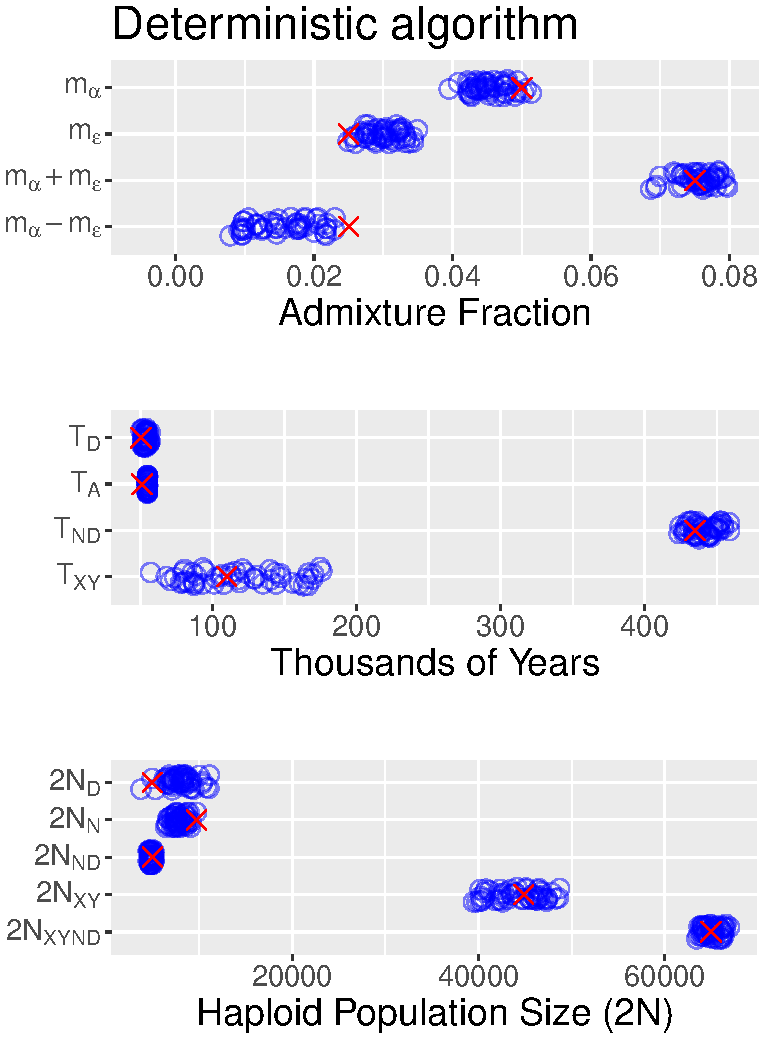
\includegraphics[width=0.5\textwidth]{det-msp-dot.pdf}\\}
  \caption{Parameter estimates from 50 simulated data sets. Blue
    circles are estimates and red crosses are the true parameter
    values. Symbols for simulation estimates have been jittered
    vertically.}
  \label{fig.dot}
\end{figure}

The code that produced this graph is on the class website in a file
called \texttt{b2.r}. For your project, modify this code to reflect
the parameter names and the true parameter values of your own
project. You may want to remove the code that graphs $m_\alpha +
m_\epsilon$ and $m_\alpha - m_\epsilon$. These were relevant to a
point I was making, but may not be of interest in your project.

Once you have edited \texttt{b2.r} as needed, you can run it from the
command line by typing \texttt{Rscript b2.r}. This will produce a file
called \texttt{b2dot.pdf}.

Here is a listing of \texttt{b2.r}:

\listinginput[3]{1}{b2.r}

\printbibliography

\end{document}
